\documentclass[tikz,border=7pt]{standalone}
\usepackage{amsmath,pgfplots}
\pgfplotsset{compat=1.18}
\definecolor{ink}{HTML}{21352F}\definecolor{teal}{HTML}{087F7B}
\definecolor{gold}{HTML}{C58B2A}\definecolor{blue}{HTML}{4B77A8}\definecolor{rose}{HTML}{B65A62}
\begin{document}
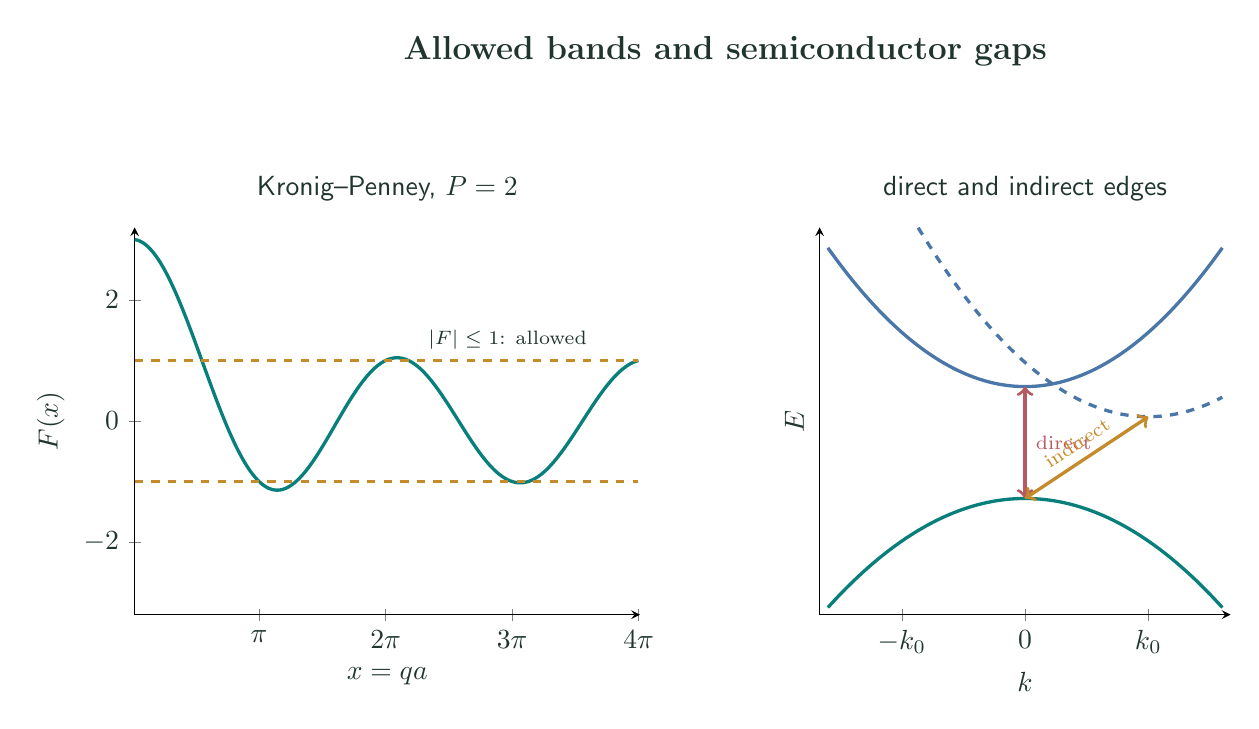
\begin{tikzpicture}[font=\sffamily,text=ink]
\node[font=\bfseries\large] at (0,4.15) {Allowed bands and semiconductor gaps};
\begin{axis}[at={(-7.5cm,-3cm)},anchor=south west,width=8cm,height=6.5cm,xmin=.05,xmax=12.6,ymin=-3.2,ymax=3.2,
 axis lines=left,xlabel={$x=qa$},ylabel={$F(x)$},xtick={3.1416,6.2832,9.4248,12.566},xticklabels={$\pi$,$2\pi$,$3\pi$,$4\pi$},title={Kronig--Penney, $P=2$}]
 \addplot[teal,very thick,domain=.05:12.56,samples=600]{cos(deg(x))+2*sin(deg(x))/x};
 \addplot[gold,dashed,thick,domain=.05:12.56]{1};
 \addplot[gold,dashed,thick,domain=.05:12.56]{-1};
 \node[font=\scriptsize,anchor=west] at (axis cs:7.1,1.35) {$|F|\leq1$: allowed};
\end{axis}
\begin{axis}[at={(1.2cm,-3cm)},anchor=south west,width=6.8cm,height=6.5cm,xmin=-2.5,xmax=2.5,ymin=-.3,ymax=4.2,
 axis lines=left,xlabel={$k$},ylabel={$E$},xtick={-1.5,0,1.5},xticklabels={$-k_0$,$0$,$k_0$},ytick=\empty,title={direct and indirect edges}]
 \addplot[blue,very thick,domain=-2.4:2.4,samples=160]{2.35+.28*x^2};
 \addplot[teal,very thick,domain=-2.4:2.4,samples=160]{1.05-.22*x^2};
 \draw[rose,<->,very thick] (axis cs:0,1.05)--(axis cs:0,2.35) node[midway,right,font=\scriptsize] {direct};
 \addplot[blue,dashed,very thick,domain=-2.4:2.4,samples=160]{2.0+.28*(x-1.5)^2};
 \draw[gold,<->,very thick] (axis cs:0,1.05)--(axis cs:1.5,2.0) node[midway,above,sloped,font=\scriptsize] {indirect};
\end{axis}
\end{tikzpicture}
\end{document}
